\section{Computer Setup}
\begin{information}
We will all be working on our own computers today, and will be accessing Virtual Machines running the Ubuntu operating system on the Nectar Research Cloud (\url{http://nectar.org.au/}).
The software client No Machine which you will have already installed, enables us to access these machines in a familiar Desktop style, even though the majority of our time will be spent within the terminal. \\
\end{information}

\begin{warning}
If you did not install NoMachine prior to today's workshop, the correct installers can be found at:
\begin{itemize}
	\item \url{http://tinyurl.com/lcn3ns8} (Windows)
	\item \url{http://tinyurl.com/mnm23ew} (Mac)
\end{itemize}
\end{warning}

\begin{information}
No Machine session files will be provided to each attendee which have been pre-configured to enable easy access to these machines.
These machines are effectively dual-core machine with 8GB of RAM \& 70GB of hard drive space.
Whilst relatively small, this will be more than enough to become familiar with the important concepts for the day.
To begin today's session, simply click (or double-click) on the No Machine session file that you have been given.
The desktop from the Virtual Machine (VM) that you have connected to will appear on the
No Machine client. \\
\end{information}

\begin{figure}[h!]
  \centering
    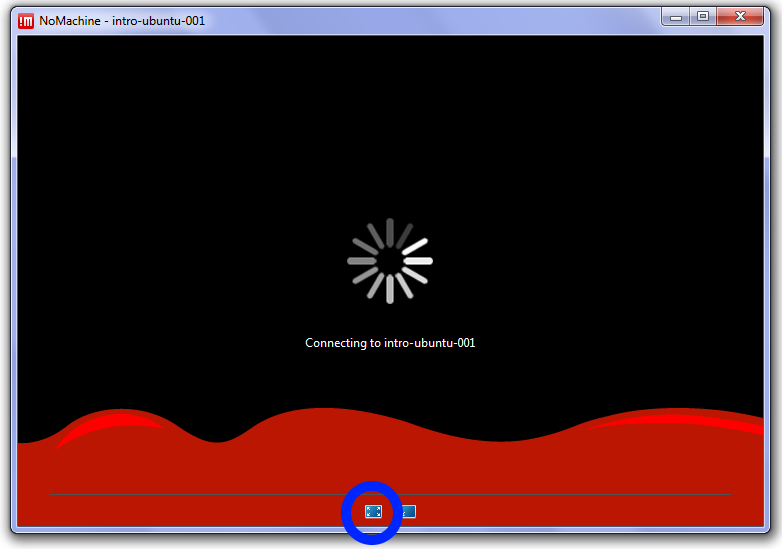
\includegraphics[width=0.8\textwidth]{images/NoMachine.png}
\end{figure}

\begin{warning}
While this is connecting, select the button circled in blue above.
This will resize NoMachine to be full screen to feel more like you are physically located at the VM.
If any security warnings appear, ignore them \& continue connecting.
This may take several attempts and if you can't connect after 3 or 4 times, call a tutor over.
\end{warning}

If you forgot to set the client to full screen, hover your mouse over the top-right corner and click where the `page' folds over. 
This will enable you to resize the client again, and can also be used to disconnect from the VM.\\


\section{The Ubuntu Desktop}
\begin{note}
Now that you are connected, you will notice we are in a standard graphical environment.
The default Desktop in Ubuntu is Unity, but what we are seeing is known as the Gnome Desktop.
It's easier to load this via NoMachine, but the two variants are not dissimilar.
As many of us are used to seeing, there are click-able icons on the desktop, and drop-down menus. \\

Although we won't be using it today, Ubuntu has an built-in Office Suite of
programs which you can access from the \textit{Applications \textgreater Office} menu item.
This is where links can be found to open Document Viewer (a .pdf viewer), Libre Office Calc (Excel-like), Libre Office Writer (Word-like) \& other standard members of Office Program Suites. \\

The two main interfaces we will be using today are the \texttt{terminal} and a text editor named \texttt{gedit}.
They will appear as icons on the desktop, but can also be accessed from the drop-down menus.
\end{note}

\subsubsection*{Firefox}

\texttt{Firefox} can also be accessed from the terminal using the command \texttt{firefox \&},  by clicking the desktop icon, or from the drop-down menu in the top left.

\begin{warning}
NB: Firefox has recently been a little unstable on these machines.
If you can't open firefox using any of the above methods it's just a small glitch as it shuts down, so call a tutor over \& they will help get the browser back up \& running.
\end{warning}